%%%
% Proposal for Alexa Fairness in AI call (Winter 2022):
%
% https://www.amazon.science/research-awards/alexa-fairness-in-ai-call-for-proposals-winter-2022
%%%

\documentclass[11pt]{article}
\usepackage[T1]{fontenc}

\usepackage{xcolor}
\definecolor{webred}{rgb}{0.5,0,0}
\definecolor{webblue}{rgb}{0,0,0.8}
\usepackage[pdftex,colorlinks,citecolor=webblue,linkcolor=webred,]{hyperref}

\usepackage{newtxmath,newtxtext}
\usepackage[letterpaper, margin=1in]{geometry}
\usepackage{setspace}
\usepackage{lipsum}
\usepackage{fancyhdr}
\usepackage{url}
\usepackage{graphicx}
\usepackage{booktabs,totpages}
\renewcommand{\arraystretch}{1.2}
\usepackage{braket}

\usepackage[final]{pdfpages}

%\input{ethos}

\usepackage[tikz]{bclogo}
\renewcommand\bcStyleTitre[1]{\centering\textbf{#1}}

\usepackage{pdfpages}
\usepackage{pgfgantt}
\usepackage{float}
\usepackage{wrapfig}
\usepackage{csquotes}

\usepackage{amsmath}
\newcommand*\diff{\mathop{}\!\mathrm{d}}

\makeatletter
\newcommand{\checkheight}[1]{%
  \par \penalty-100\begingroup%
  \setbox8=\hbox{#1}%
  \setlength{\dimen@}{\ht8}%
  \dimen@ii\pagegoal \advance\dimen@ii-\pagetotal
  \ifdim \dimen@>\dimen@ii
    \break
  \fi\endgroup}
\makeatother

\newcommand{\meansl}{[\![}
\newcommand{\meansr}{]\!]}
\newcommand{\means}[1]{\meansl #1 \meansr}
\newcommand{\reals}{\mathbb{R}}                    %reals
\newtheorem{definition}{Definition}
\newcommand{\tup}[1]
{
 \relax\ifmmode
 \langle #1 \rangle
 \else $\langle$ #1 $\rangle$ \fi
}

\pagestyle{fancy}
\fancyhf{} % sets both header and footer to nothing
\renewcommand{\headrulewidth}{0pt}
\cfoot{Page \thepage}

\DeclareRobustCommand{\rchi}{{\mathpalette\irchi\relax}}
\newcommand{\irchi}[2]{\raisebox{\depth}{$#1\chi$}} % inner command, used by \rchi

%\linespread{1.3}

% \usepackage{etoolbox}
% \patchcmd{\thebibliography}
%   {\settowidth} % a little space instead of 0pt in next: 0pt plus 0.1pt
%   {\setlength{\itemsep}{-0.25em}\settowidth}
%   {}{}
% \apptocmd{\thebibliography}
%   {\small}
%   {}{}

\begin{document}
\title{Provable Fairness for Natural Language Models \\ using Neural Network Formal Verification \\
{\large Proposal for Alexa Fairness in AI Amazon Research Award (Winter 2022)}}
\author{
}
\date{}
\maketitle

\thispagestyle{fancy}

\vspace{-2em}
\noindent
\textbf{PI:} Stanley Bak, Assistant Professor, Computer Science, Stony Brook University

\noindent
\textbf{Co-PI:} Steven Skiena, Empire Innovation Professor, Computer Science, Stony Brook University

\noindent
\textbf{Cash Funding Needed:} \$80K

\noindent
\textbf{AWS Promotional Credits Needed:} \$10K


\begin{abstract}

\noindent
Machine learning models are increasingly deployed for important decision-making tasks, making it important to verify that they do not contain gender or racial biases picked up from training data.
%
Typical approaches to achieve fairness revolve around efforts to clean or curate training data, with post-hoc statistical evaluation of the fairness of the model on evaluation data.

\vspace{1em}
\noindent
In contrast, we propose techniques to \emph{prove} the fairness properties using recently developed formal methods that verify properties of neural network models.
%
Beyond the strength of guarantee implied by a formal proof, our methods have the advantage that we do not need explicit training or evaluation data (which is often proprietary) in order to analyze a given trained model.
%
The research focus is on extending formal verification approaches to long short-term memory (LSTM) networks, as well as a systematic classification of formal fairness specifications that can be proven about a given network.

\vspace{1em}
\noindent
\textbf{Keywords:} Neural Network Verification, Provable Fairness, LSTM
\end{abstract}

\section*{Introduction}
% Significance of the research and prior work.   

\noindent
Formal approaches to neural network verification have been developed over the past few years~\cite{liu2019algorithms,tran2020verification,katz2017reluplex,gehr2018ai2} that can in certain cases prove properties about all possible executions of a specific network.
%
Existing work has focused on networks used in safety-critical control algorithms and robotics~\cite{ivanov2019verisig,xiang2020reachable}, or guaranteed robustness for visual perception networks~\cite{tran2019safety}.
%
We propose to extend such methods---specifically those based on star set overapproximations~\cite{tran2020verification}---to network architectures commonly used in natural language processing (NLP), such as gated recurrent unit (GRU) networks and long short-term memory (LSTM) networks~\cite{xingjian2015convolutional}.
%
In addition, we plan to systematically explore classes of fairness specifications that can be evaluated both statistically as well as using the developed formal approaches.
%
If successful, the project will extend highly-accurate formal verification methods to support GRU and LSTM cells.

NLP networks and enable the possibility of evaluating a given network with respect to different definitions of fairness.
%
Further, such fairness definitions could be embedded into the training process help create fair NLP systems, similar to methods for formal verification of perception systems have been used to create more robust vision systems.

\vspace{1em}
\noindent
\textbf{Prior Work on LSTM and Transformer Verification. } Many approaches have emerged in recent years for neural network verification, and the PI helps run an annual competition to evaluate method applicability and scalability~\cite{vnncomp2021}.
%
Despite progress, less work has been done on generalizing analysis methods to architectures and layers using in LSTM, due to complexity and nonlinearity.
%
Some coarse analysis methods exist for recurrent and LTSM neural networks, such as those based on interval bounds~\cite{jia2019certified}, single upper and single lower linear function bounds~\cite{ko2019popqorn,shi2020robustness}, bounding planes~\cite{du2021cert}, polyhedral abstractions from samples~\cite{ryou2021scalable}, and multi-norm zonotopes~\cite{bonaert2021fast}.
%
Our approach, in contrast is based on efficient geometric data structures called linear star sets~\cite{duggirala2016parsimonious}, which have been used by the PI in formal verification methods for cyber-physical systems~\cite{bak2017hscc,bak2019hscc} and also extended to ReLU neural networks~\cite{tran2019star,bak2020cav,bak2021nnenum}.
%
The advantage of this method compared with the existing approaches is the potential for higher accuracy---arbitrary linear constraints can be used to construct tight bounds on the nonlinear layers.

In our initial experiments, such methods are essential for creating tight bounds for softmax and self-attention layers.
%
A figure of a prototype implementation showing linear bounds of a softmax layer is shown in Figure~\ref{fig:softmax}, where the true nonconvex output is in blue, and the outer convex linear bounds using the star set representation are shown.
%
Based on this promising progress, we plan to integrate the approach into an open-source tool for proving fairness properties in LSTM networks, such as the PIs \texttt{nnenum} tool\cite{bak2021nnenum} which is available online\footnote{\url{https://github.com/stanleybak/nnenum}} but currently only verifies ReLU networks.

\begin{figure}[t]
    \centering
    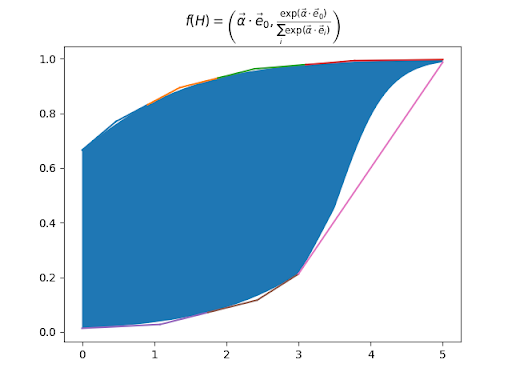
\includegraphics[width=0.5\columnwidth]{figs/softmax.png}
    \caption{The star set approach can provide tight bounds on nonlinear layers such as softmax. The blue set is the real possible outputs of a neuron, projected onto the input ($x$ axis) and output ($y$ axis) of a single neuron.}
    \label{fig:softmax}
\end{figure}

\vspace{1em}
\noindent
\textbf{Prior Work on Proving Fairness. } 
%
A limited amount of existing research also exists on provable fairness.
%
One framework focuses on proving \emph{dependency
fairness}~\cite{urban2020perfectly,galhotra2017fairness}, which strives to prove the outputs are not affected by certain input features.
%
This method is based on forward and a backward static analysis as well as input feature partitioning.
%
The star set approach, in contrast, performs overapproximation and partitioning based on the nonconvexity in the activation functions, and so is likely to have improved scalability to larger networks or input spaces.

Another recent approach~\cite{ruoss2020learning} focuses on \emph{individual fairness}, which essentially means that similar individuals get similar treatments.
%
In this case, the verification approach uses mixed integer linear programming (MILP), which can be as accurate as star sets, but in our experience with ReLU networks is often significantly less scalable in terms of network size and analysis time.

\section*{Methods}

Our technical approach to verification is based on set-based execution of neural networks, extended to include probability distributions.
%
Given a set of possible inputs, we propagate the set through the network to see the range of the network, the possible outputs.
%
This process requires choosing representations for a set of states, with operations defined how the set transforms based on each layer in the network.
%
In our proposed approach, we will use the linear star set representation~\cite{duggirala2016parsimonious,tran2020cav} to represent sets of states, which we simply call star sets.
%
A star set is an affine trasnformation of a half-space polytope, where the affine transformation and polytope terms are kept separate.
%
A star set $\Theta$ defines a set of states as $\Theta  = \{x \in \mathbb{R}^n ~ | ~ \exists {\alpha \in \mathbb{R}^m}, ~ x = V \alpha + c \wedge C\alpha \leq d\}$. 
%
This representation is useful for neural network verification because operations such as affine transformation, intersection, and optimization are accurate and efficient even in high-dimensional sets, corresponding to layers in a neural network with a large number of neurons.
%
At the end of analysis, the entire input set is partitioned into a number of star sets, where each star set $\Theta$ maps a half-space polytope in the domain $\mathcal{D}$ (defined by $C\alpha \leq d$), to outputs with an identical label.

\begin{figure}[t]
    \centering
    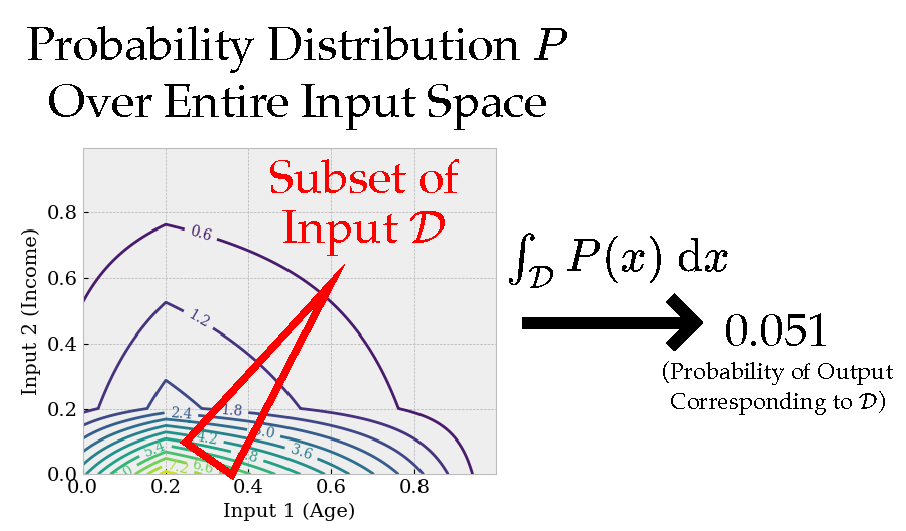
\includegraphics[width=0.6\columnwidth]{figs/fairness_image.pdf}
    \caption{Each partition $\Theta$ of the network input space is used as the domain for integration over a given input probability density function $P$, calculating a probability of the input space with a fixed output classification. 
    %
    Repeating and summing over all partitions, we can evaluate fairness metrics for the network.}
    \label{fig:input_split}
\end{figure}

We plan to extend existing set propagation methods with star sets to work with layers in LSTM networks, and then using the result to reason over how probability distributions can be propagated through the network.
%
%The output of this analysis is a partition of the inputs space into star sets, where every input point in each partition classifies the same way.
%
Given a subset of the input space represented as a polytope in the domain $\mathcal{D}$ with a corresponding single output label, we can compute the probability density corresponding to that label integrating over the input domain, $\int_\mathcal{D} P(x) ~ \diff x$, where the probability density function $P(x)$ is defined over the entire input space.
%
Repeating this over the entire input domain (all the star set partitions), we can compute the probability of each output over the entire domain of possible inputs.
%
The process is illustrated in Figure~\ref{fig:input_split} on a hypothetical 2-d input distribution, where a single partition over the input space given as a polytope $\mathcal{D}$ is used to compute a probability of a specific output.

The definition of fairness we strive to prove is then based on the calculated probability distributions.
%%%%%%%%%%%%%%%%%%%%55
%
We will consider the following types of fairness challenges that can be verified using formal methods:

\begin{itemize}
\item \textbf{Classification with explicit input labels.} Here one of the input fields for each record explicitly encodes a sensitive property, such as race, gender, or age.   Fairness dictates that a given model M performs “the same’’ for all possible values of these sensitive fields.
%
\item \textbf{Classification with differential input distributions.} Here sensitive information is not explicitly passed to the model but may be inferable from other input variables (e.g. the zip code of an African-American neighborhood).   In addition to a given model M we are given input probability distributions for two or more distinct groups.   Fairness dictates that M performs “the same” over records drawn from these distinct input distributions.
\end{itemize}

Every binary decision model partitions the space of possible inputs into a collection of geometric polytopes, such that all points within any particular polytope $\mathcal{D}$ are labeled homogeneously as all positive or all negative. 
%
The fairness properties which we are concerned with revolve around showing that these geometric regions are comparable for two distinct labels or groups. There are several possible provable properties depending upon how we define that M performs “the same” for different groups, including:  

\begin{itemize}
\item \textbf{Volumetric identity.}  Here we say that M is provably fair when the positive regions are identical for different groups A and B, ignoring the input variable explicitly encoding the identity of group A and B.
Volumetric magnitude – Here we say M is provably fair when the volume of the positive regions are comparable for different groups A and B.   The symmetric difference of the positive regions of A and B may be greater than zero, but the difference of the size of the input volumes is provably bounded.
%
\item \textbf{Probability-weighted magnitude.}  Here we say that M is provably fair with respect to input distributions A and B when the weighted volumes of the positive regions are the same for A and B, or that the difference of these weighted volumes is provably bounded.  The weighted volume of polytope $\mathcal{D}$ is defined by the integral of the probability of each point in $\mathcal{D}$.
\end{itemize}

%Add the notion of threshold invariant models, where these ideas hold over all decision boundary thresholds (not just >= 0.5).


\section*{Expected Results}
% Please include milestones with timeline estimates, such as for datasets, code releases, technical reports, publications, applications, presentations, etc. 
We anticipate open-source code releases with the work, along with publications related to the basic research and associated presentations.
%
The code will be continuously released on github and publications will likely become available during the second half of the project, in Spring 2023.
%
At this point we anticipate 2-3 publications related to the basic research and tool implementation of the developed methods.
%
Presentations and publications will be made available online for widest dissemination of research results.
%
In addition to the direct products of the work, we anticipate some of the fairness specifications can be interested into the neural network verification competition run by the PI~\cite{vnncomp2021}.
%
In this way, the work can leverage research effort by other groups around the world to develop methods to address fairness concerns in NLP systems.

\section*{Funds Needed}
% Please provide justification supporting the designated amounts for cash funding and AWS Promotional Credits. For cash funding, please do not include indirect expenses which are not incurred solely for your project. For AWS Promotional Credits, please list the AWS products you plan to use.
For the project we plan to fund two graduate students as research assistants. %
Each of the three semesters (including summer) costs \$11K, with \$2826 tuition for Spring and Fall. The total direct costs for salary is 2 students * 3 semesters * \$11K + 2 students * 2 semesters * \$2826 = \$77304. We also plan to allocate \$2696 for domestic travel to conferences related to formal methods and verification such as CAV or NeurIPS.

For Amazon promotional credits, we are requesting \$10K. In past research, our group has used EC2 to evaluate verification approaches using EC2 instances both with powerful CPUs and GPUs, and we anticipate this project will require similar resources for development and evaluation for fairness verification techniques.

\section*{Additional Information}
%PIs are encouraged to exemplify how their proposed techniques or research studies will apply to tasks in natural language understanding, natural language generation, speech and speaker recognition and/or computer vision. PIs should either include plans for open source contributions or state that they do not plan to make any open source contributions (data or code) under the proposed effort.

Our proposed improvements to verification methods are targeted to layers and architectures used for NLP systems.
%
We plan to integrate research developments into the PI's open source verification tool, \texttt{nnenum}, which currently only supports analysis of ReLU networks without probability distributions over the inputs.


\bibliographystyle{abbrv}
\bibliography{refs}
% References Limit two pages.

\appendix

\clearpage
%\textcolor{red}{TODO: re-add includepdf command here to insert CVs!!! (probably need to download project locally since it's timing out)}
\thispagestyle{empty}
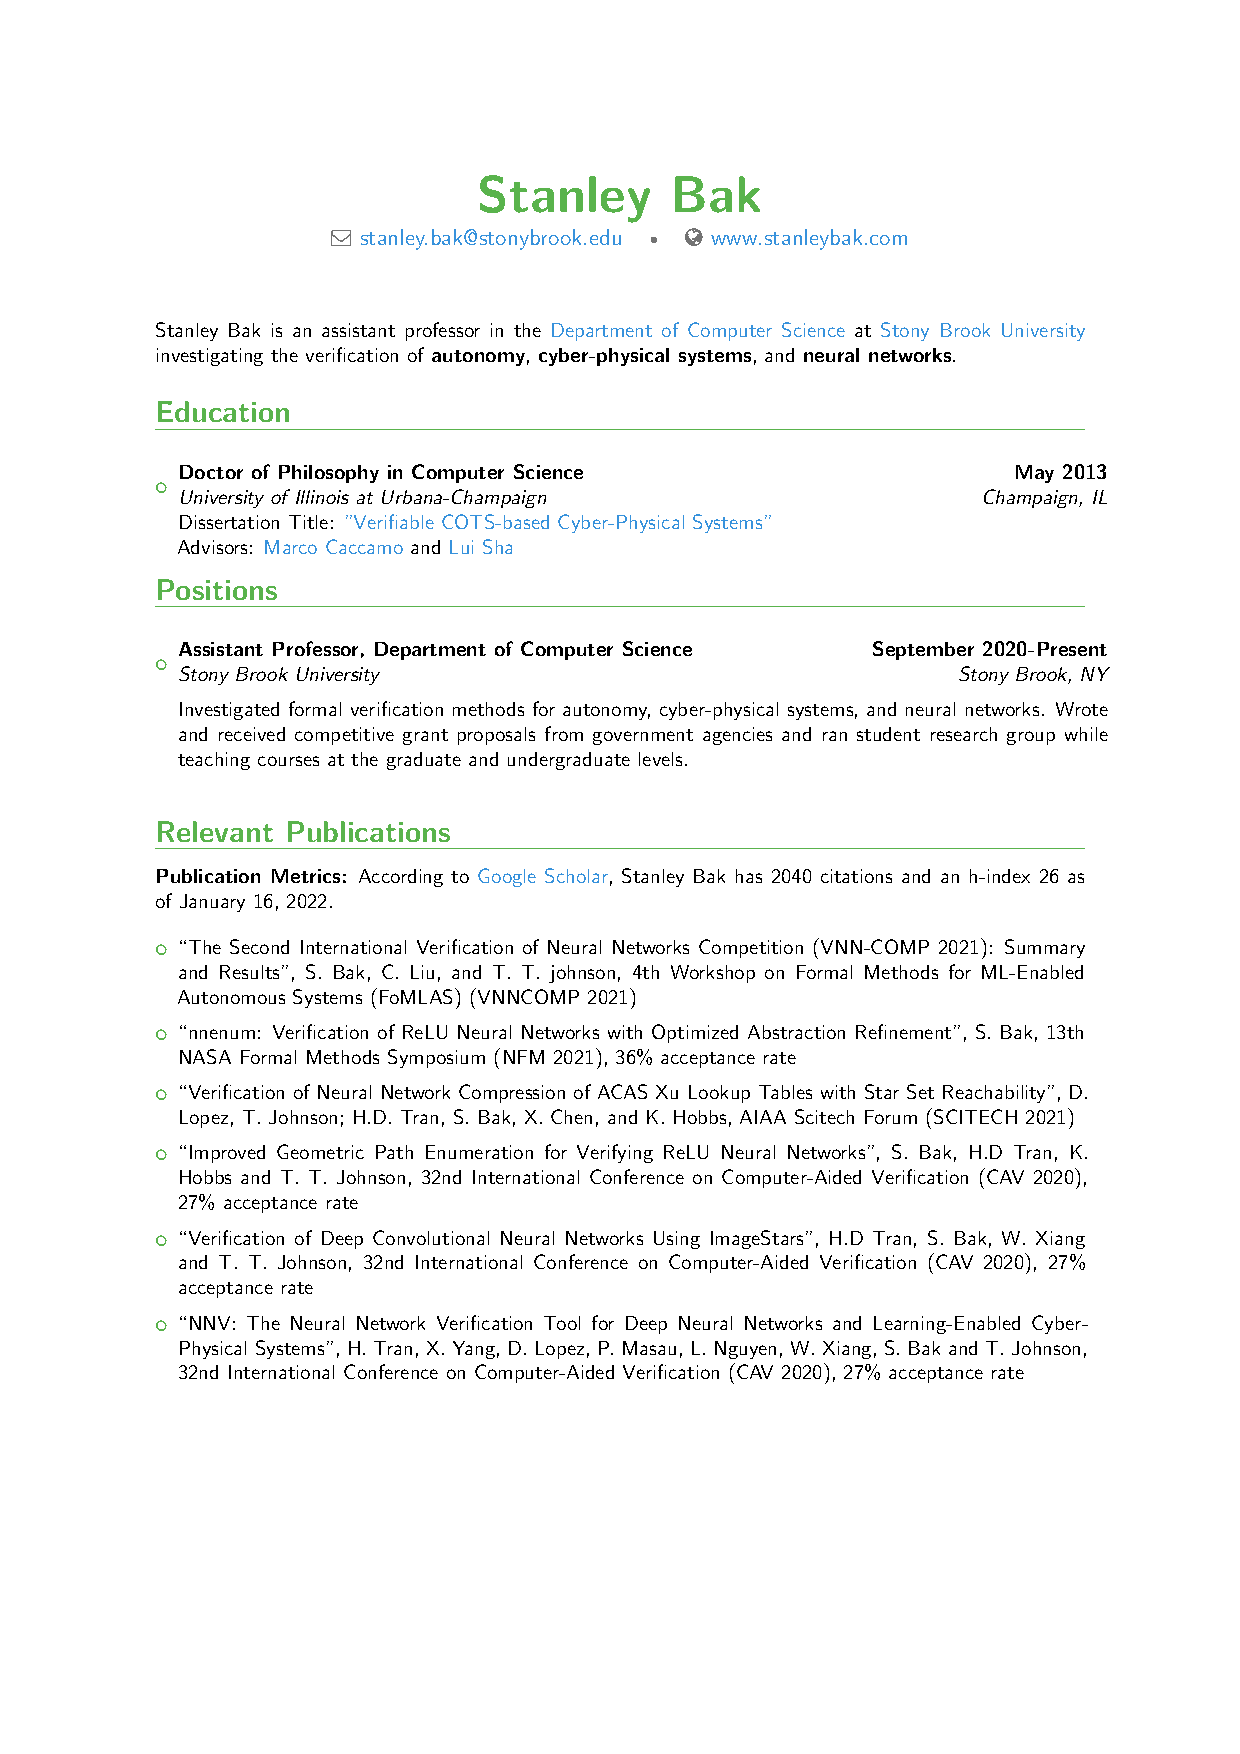
\includepdf{cv/cv-bak.pdf}

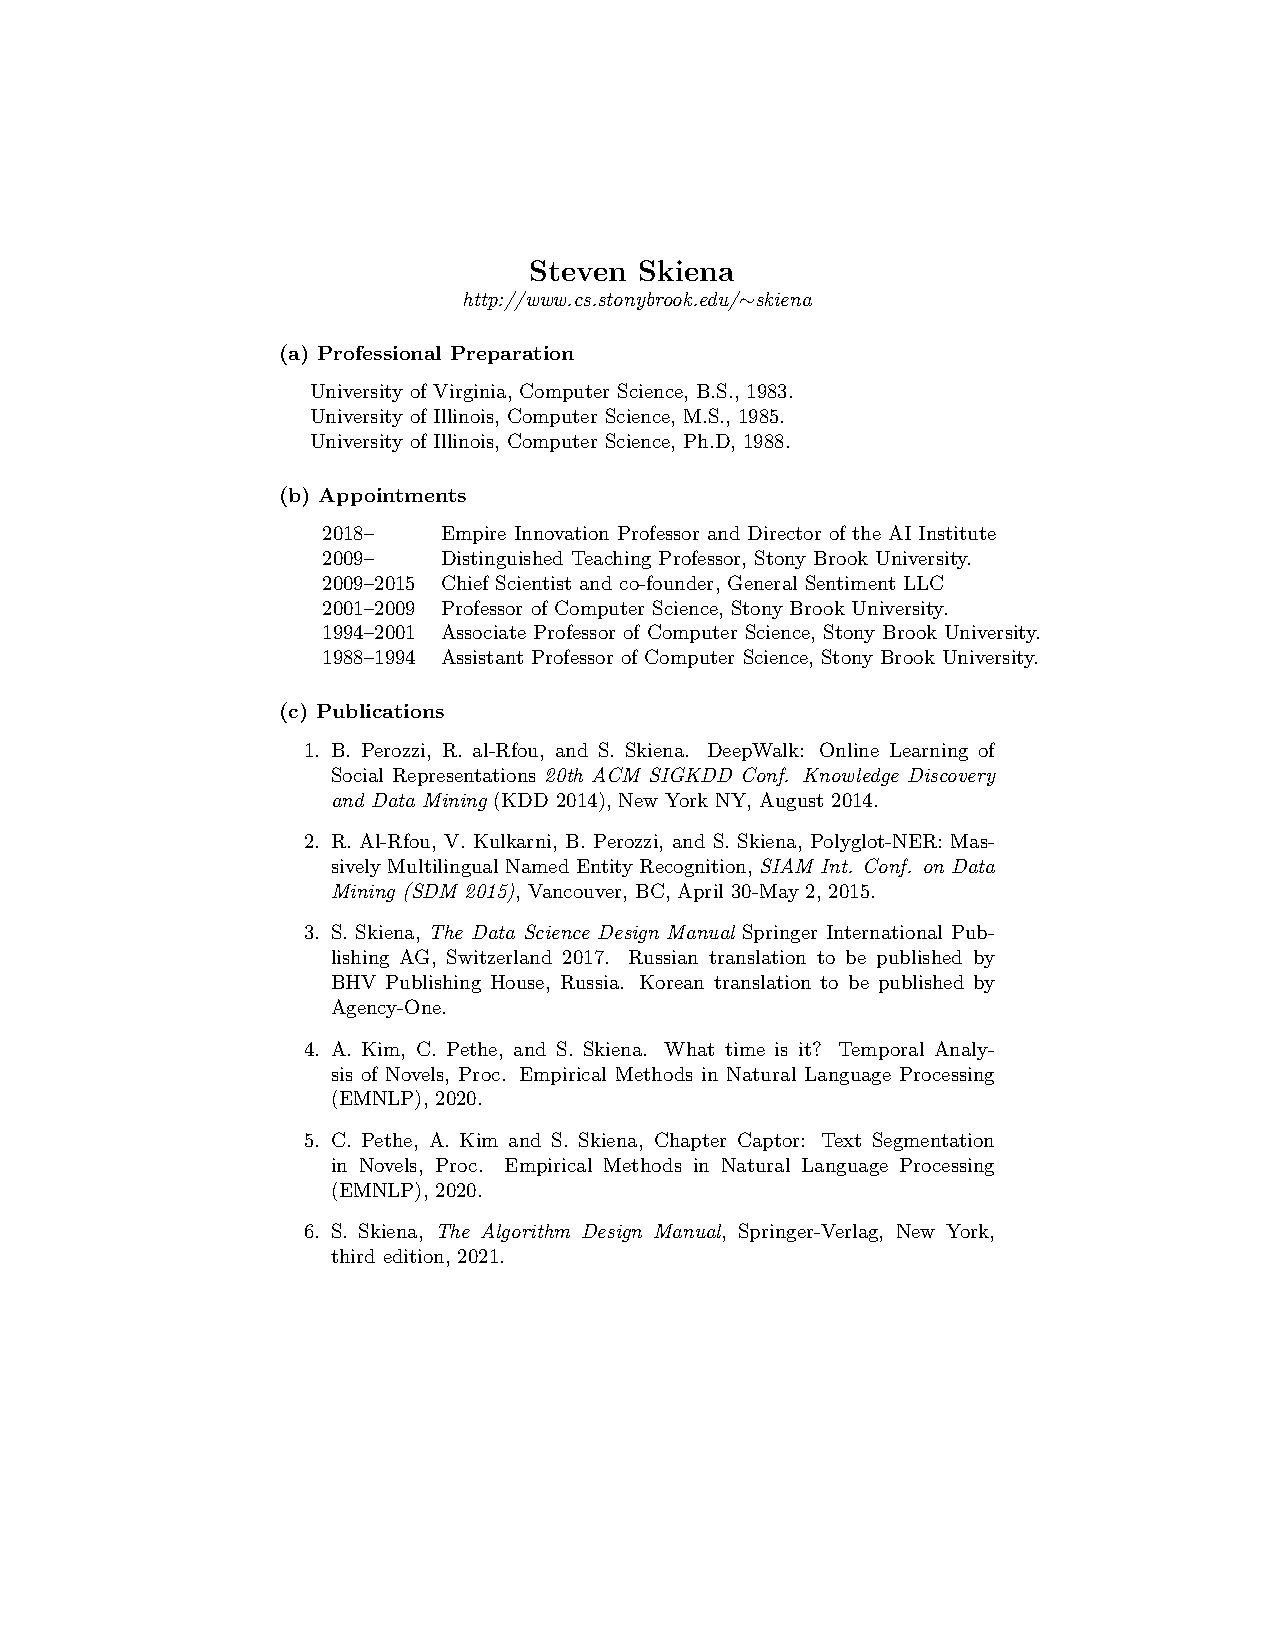
\includepdf{cv/cv-skiena.pdf}

\clearpage
\section*{Previously Funded Project Summary}
Neither the PI and co-PI do not have previous funded projects with Amazon within the past 3 years.

%also attach CV

\end{document}
